\documentclass{article}
\usepackage{amsmath,amsthm,amssymb,amsfonts}
\usepackage{setspace,enumitem}
\usepackage{graphicx}
\usepackage{hyperref}
\usepackage{natbib}
\usepackage{afterpage}
\usepackage{xcolor}
\usepackage{etoolbox}
\usepackage{booktabs}
\usepackage{pdfpages}
\usepackage{multicol}
\usepackage{geometry}
\usepackage{accents}
\usepackage{bbm}
\usepackage{placeins}
\usepackage{verbatim}
\usepackage{lscape}
\usepackage{csvsimple}
\hypersetup{
	colorlinks,
	linkcolor={blue!90!black},
	citecolor={red!90!black},
	urlcolor={blue!90!black}
}

\newtheorem{theorem}{Theorem}
\newtheorem{assumption}{Assumption}
\newtheorem{definition}{Definition}
\newtheorem{lemma}{Lemma}
\setlength{\parindent}{0cm}
\geometry{margin = 1in}

\newcommand{\R}{\mathbb{R}}
\newcommand{\ubar}[1]{\underaccent{\bar}{#1}}
\newcommand{\Int}{\text{Int}}
\newcommand{\xbf}{\mathbf{x}}
\newcommand{\Abf}{\mathbf{A}}
\newcommand{\Bbf}{\mathbf{B}}
\newcommand{\Gbf}{\mathbf{G}}
\newcommand{\bbf}{\mathbf{b}}
\newcommand{\one}{\mathbbm{1}}

\newtoggle{extended}
\settoggle{extended}{false}

\title{ECON 717B: PS 1}
\author{Alex von Hafften}

\begin{document}

\maketitle

\section{Part 1: Analytic Exercises}

\begin{enumerate}

\item Returns to schoolings

\begin{enumerate}

\item ATE

Marginal treatment effect is

$$
MTE(A) = Y_1(A) - Y_0(A) = 1 + 0.5A - A = 1 - 0.5A
$$

Average treatment effect is

$$
E[MTE(A)] = E[1 - 0.5A] = 1 - 0.5E[A] = 1 - 0.5*0.5 = 0.75
$$

\item Fraction of treated population

$$
Pr\{D = 1\} = Pr\{-0.5 + A > 0 \} = Pr\{A > 0.5 \} = 0.5
$$

\item Maximum and minimum treatment effect

$$
\max_{A \in [0,1]} MTE(A) = \max_{A \in [0,1]} [1 - 0.5A] = 1
$$

at $A = 0$.

$$
\min_{A \in [0,1]} MTE(A) = \min_{A \in [0,1]} [1 - 0.5A] = 0.5
$$

at $A = 1$.


\item $A \sim N(0, 1)$

$$
\sup_{A \in (-\infty,\infty)} MTE(A) = \sup_{A \in (-\infty,\infty)} [1 - 0.5A] = \infty
$$

as $A \to -\infty$.

$$
\inf_{A \in (-\infty,\infty)} MTE(A) = \inf_{A \in (-\infty,\infty)} [1 - 0.5A] = -\infty
$$

as $A \to \infty$.

\item ATET and ATEU

$$
ATET = E[MTE(A) | D = 1] = E[1- 0.5A | A > 0.5] = 1- 0.5 E[A | A > 0.5] = 1 - 0.5*0.75 = 0.625
$$

$$
ATEU = E[MTE(A) | D = 0] = E[1- 0.5A | A < 0.5] = 1- 0.5 E[A | A < 0.5] = 1 - 0.5*0.25 = 0.875
$$

\item Why is ATEU $>$ ATET?

ATEU $>$ ATET because the marginal treatment effect is decreasing in $A$, but selection into treatment is increasing in $A$.

\item OLS estimand

$$
\beta(OLS) = E[Y|D=1] - E[Y|D=0] = E[1 + 0.5A |A > 0.5] - E[A|A < 0.5] = 1 + 0.5 *0.75 - 0.25 = 1.125
$$

\item Why is OLS biased upward for ATE?

Because conditional independence fails due to selection effects.  If treatment was random, then OLS would be unbiased.

\end{enumerate}

\item Monotonicity

\begin{enumerate}

\item Prove monotonicity holds.

For each observation $i$, define $V_{0,i} \equiv \delta_0 + U_{V,i}$ as the outcome without treatment and $V_{1,i} \equiv \delta_0 + \delta_1 + U_{V,i}$ as the outcome with treatment.

Case 1: $\delta_1 > 0 \implies \delta_0 + \delta_1 + U_{V,i} > \delta_0 + U_{V,i} \implies V_{1,i} > V_{0,i}$ for all $i$. Monotonicity holds.

Case 2: $\delta_1 < 0 \implies \delta_0 + \delta_1 + U_{V,i} < \delta_0 + U_{V,i} \implies V_{1,i} < V_{0,i}$ for all $i$. Monotonicity holds.

Case 3: $\delta_1 = 0 \implies\delta_0 + \delta_1 + U_{V,i} = \delta_0 + U_{V,i} \implies V_{1,i} = V_{0,i}$ for all $i$. Monotonicity holds.

\item Define $V$ such that monotonicity fails.

Consider heterogenous $\delta_{1,i} \in [-A, A]$:

$$
V_i = \delta_0 + \delta_{1,i} Z_i + U_{V, i}
$$

Since $\delta_{1,i}$ can be positive or negative, defier will not choose the treatment even if they are exposed to the instrument.

\end{enumerate}

\item Potential outcomes with uniform instrument

\begin{enumerate}

\item Show range of always takers, compliers, defiers, and never takers.

Monotonicity holds, so there are no defiers. Always takers have $V > 0$ for both $Z = 0$ and $Z = 1$, so $U_V \in [0, 2]$. Compliers $V > 0$ for $Z = 1$, but $V < 0$ for $Z = 0$, so $U_V \in [-1, 0)$. Never takers have $V < 0$ for both $Z = 0$ and $Z =1$, so $U_V \in [-2, -1)$. The figure below summarizes these ranges:

\begin{center}
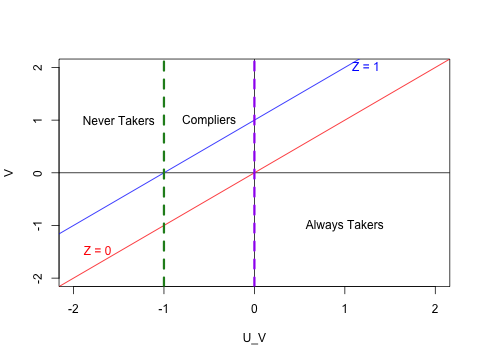
\includegraphics[scale = 0.8]{p1_q3_a}
\end{center}

\item Compute fraction of population in each group.

Using the uniform distribution, defiers are 0 percent, always takers are 50 percent, compliers are 25 percent, and never takers are 25 percent.

\end{enumerate}

\item Two types

\begin{enumerate}

\item Compute ATE

\begin{align*}
ATE 
&= E[\Delta]\\
&= Pr(Type 1) E[\Delta | Type 1] + Pr(Type 2) E[\Delta | Type 2] \\
&= (0.3) (2) + (0.7) (-1) \\
&= -0.1
\end{align*}

\item Compute $Pr(D=1 | Z = 1)$ and $Pr(D=1 | Z = 0)$

\begin{align*}
Pr(D=1 | Z = 1)
&= Pr(D=1 | Z = 1, Type 1)Pr(Type 1) + Pr(D=1 | Z = 1, Type 2)Pr(Type 2) \\
&= P(1+ U_V > 0)(0.3) + P(2+ U_V > 0)(0.7) \\
&= (1.0)(0.3) + (1.0)(0.7) \\
&= 1.0
\end{align*}

\begin{align*}
Pr(D=1 | Z = 0)
&= Pr(D=1 | Z = 0, Type 1)Pr(Type 1) + Pr(D=1 | Z = 0, Type 2)Pr(Type 2) \\
&= P(U_V > 0)(0.3) + P(U_V > 0)(0.7) \\
&= (0.5)(0.3) + (0.5)(0.7) \\
&= 0.5
\end{align*}

\pagebreak

\item Compute LATE

Notice that compliers of both Type 1 and Type 2 have $U_V \in [-1, 0]$

\begin{align*}
LATE 
&= E[\Delta | U_V < 0]\\
&= Pr(Type 1) E[\Delta | U_V < 0, Type 1] + Pr(Type 2) E[\Delta | U_V < 0, Type 2]\\
&= (0.3)(2.0) + (0.7)(-1.0)\\
&= -0.1
\end{align*}

\end{enumerate}
\end{enumerate}
\begin{landscape}

\section{Monte Carlo Exercises}

\subsection{Question 1}

\begin{enumerate}

\item See \texttt{p2\_q1.do}.

\item See table below.

\item  $z_1$ and $z_2$ are valid instruments because they affect schooling $s$ (i.e. relevance) but they do not affect log wages except through schooling (i.e. exogeneity). $z_3$ is not a valid instrument because it does not affect schooling (i.e., it fails relevance). $z_1$ is likely a weak instrument because its variance is relatively small.

\item See table below.

\begin{tabular}{lccccccc} \hline
 & (1) & (2) & (3) & (4) & (5) & (6) & (7) \\
VARIABLES & 2SLS & 2SLS & 2SLS & 2SLS & 2SLS & 2SLS & 2SLS \\ \hline
 &  &  &  &  &  &  &  \\
s & 0.0589*** & 0.0501*** & -0.0202 & 0.0501*** & 0.0501*** & 0.0531*** & 0.0501*** \\
 & (0.0170) & (0.000573) & (0.222) & (0.000573) & (0.000573) & (0.0164) & (0.000573) \\
Constant & 1.000*** & 1.004*** & 1.036*** & 1.004*** & 1.004*** & 1.002*** & 1.004*** \\
 & (0.0158) & (0.0142) & (0.114) & (0.0142) & (0.0142) & (0.0158) & (0.0142) \\
 &  &  &  &  &  &  &  \\
Observations & 2,000 & 2,000 & 2,000 & 2,000 & 2,000 & 2,000 & 2,000 \\
R-squared & 0.866 & 0.857 &  & 0.857 & 0.857 & 0.864 & 0.857 \\
Instruments & z\_1 & z\_2 & z\_3 & z\_1 z\_2 & z\_2 z\_3 & z\_1 z\_3 & z\_1 z\_2 z\_3 \\
 F-Statistic & 1.711 & 8154 & 0.130 & 4075 & 4075 & 0.926 & 2716 \\ \hline
\multicolumn{8}{c}{ Standard errors in parentheses} \\
\multicolumn{8}{c}{ *** p$<$0.01, ** p$<$0.05, * p$<$0.1} \\
\end{tabular}


\item The OLS estimate is biased upward for $\beta_2$.  Including just $z_1$ exacerbated the bias likely due it being a weak instrument. Including just $z_2$ reduces the bias and boosts the first stage F-statistic. Including just $z_3$, the results are way off which makes sense because it is not a relevant instrument. Any of the combinations that include $z_2$ do well, but without $z_2$ does poorly. Including all three instruments lowers the F-statistics.  This table suggest that we would want to include just $z_2$ or both $z_1$ and $z_2$.

\pagebreak

\item See table below for $N = 500,000$.

\begin{tabular}{lccccccc} \hline
 & (1) & (2) & (3) & (4) & (5) & (6) & (7) \\
VARIABLES & 2SLS & 2SLS & 2SLS & 2SLS & 2SLS & 2SLS & 2SLS \\ \hline
 &  &  &  &  &  &  &  \\
s & 0.0477*** & 0.0500*** & 0.0557*** & 0.0500*** & 0.0500*** & 0.0498*** & 0.0500*** \\
 & (0.0124) & (3.62e-05) & (0.0194) & (3.62e-05) & (3.62e-05) & (0.0103) & (3.62e-05) \\
Constant & 0.999*** & 0.999*** & 0.999*** & 0.999*** & 0.999*** & 0.999*** & 0.999*** \\
 & (0.00108) & (0.000905) & (0.00122) & (0.000905) & (0.000905) & (0.00102) & (0.000905) \\
 &  &  &  &  &  &  &  \\
Observations & 500,000 & 500,000 & 500,000 & 500,000 & 500,000 & 500,000 & 500,000 \\
R-squared & 0.845 & 0.854 & 0.865 & 0.854 & 0.854 & 0.854 & 0.854 \\
Instruments & z\_1 & z\_2 & z\_3 & z\_1 z\_2 & z\_2 z\_3 & z\_1 z\_3 & z\_1 z\_2 z\_3 \\
 F-Statistic & 3.688 & 2.151e+06 & 1.317 & 1.075e+06 & 1.075e+06 & 2.504 & 716915 \\ \hline
\multicolumn{8}{c}{ Standard errors in parentheses} \\
\multicolumn{8}{c}{ *** p$<$0.01, ** p$<$0.05, * p$<$0.1} \\
\end{tabular}


\end{enumerate}

\end{landscape}

\subsection{Question 2}

\begin{enumerate}

\item See \texttt{p2\_q2.jl}

\item ATE is 2.992, ATET is 3.179, ATEU is 2.869, OLS/Naive estimator is 3.397, direct/reduced form/ITT estimator is 2.359, and IV estimator is 2.873.

\item Fraction of compliers is 0.8216.

\item  ATE is 2.995, ATET is 3.275, ATEU is 2.837, OLS/Naive estimator is 3.568, direct/reduced form/ITT estimator is 2.029, and IV estimator is 2.974. Fraction of compliers is 0.6863.

\end{enumerate}

\end{document}